\documentclass{article}

\usepackage{neurips_2026}

\usepackage[utf8]{inputenc}
\usepackage[T1]{fontenc}
\usepackage{hyperref}
\usepackage{url}
\usepackage{booktabs}
\usepackage{amsfonts}
\usepackage{amsmath}
\usepackage{amssymb}
\usepackage{nicefrac}
\usepackage{microtype}
\usepackage{xcolor}
\usepackage{graphicx}
\usepackage{multirow}
\usepackage{algorithm}
\usepackage{algorithmic}

\title{GRAPE: Graph-Augmented Prototype Explanations for\\
Trustworthy Medical Image Diagnosis}

\author{%
  Anonymous Authors\\
  Anonymous Institution\\
  \texttt{anonymous@example.com}
}

\begin{document}

\maketitle

\begin{abstract}
Interpretable medical image classifiers must be both accurate and trustworthy: every prediction should be traceable to clinically meaningful visual evidence, and every doctor interaction should be safe.
Existing prototype-based models treat clinical concepts as independent, ignore the risk of unsafe doctor feedback, and require full retraining to add new findings.
We present \textbf{GRAPE} (Graph-Augmented Prototype Explanations), a new architecture that addresses all three limitations simultaneously.
GRAPE introduces: (i) a \emph{Graph Attention Task Head} that models anatomical concept co-occurrence via a learned GAT over concept similarity scores, replacing the flat linear classifier; (ii) \emph{Uncertainty-Aware Spatial Interaction}, which computes per-patch prototype variance maps and issues a safety warning before amplifying uncertain or misattributed spatial feedback; and (iii) \emph{Open-Vocabulary Prototype Anchoring}, which aligns visual concept prototypes to frozen BioViL-T text embeddings during training, enabling zero-shot addition of new clinical concepts without retraining.
Trained with a four-stage pipeline combining concept supervision, multi-prototype contrastive learning, cross-modal alignment, and graph-structured classification, GRAPE achieves \textbf{+14.4\%} macro-F1 over the prototype baseline on TBX11K (3-class TB detection) and \textbf{+9.7\%} on NIH ChestX-ray14 (14-concept binary classification), while improving Pointing Game accuracy by up to \textbf{+12.3 pp}.
At batch size 1, the GAT head adds only 1~ms latency, satisfying real-time interaction requirements.
\end{abstract}

%% ─────────────────────────────────────────────────────────────────
\section{Introduction}
\label{sec:intro}
%% ─────────────────────────────────────────────────────────────────

Deep learning has achieved radiologist-level accuracy on several medical imaging tasks~\cite{rajpurkar2017chexnet,chen2020tbx11k}, yet clinical adoption remains limited. Two barriers stand out. First, black-box models provide no evidence for their predictions, making it impossible for a physician to verify or override the reasoning. Second, even ``interpretable'' models may silently propagate spatial errors when doctors provide corrective feedback, creating a patient-safety risk.

Prototype-based models~\cite{chen2019looks,donnelly2022deformable} address the first barrier by making predictions through similarity to learned visual examples. Recent work on Concept-based Similarity Reasoning (CSR)~\cite{csr2025} extends this to multi-prototype per-concept reasoning with doctor-in-the-loop interaction. However, three structural limitations remain:

\begin{enumerate}
    \item \textbf{Independent concepts.} The task head is a flat linear layer applied to concatenated concept similarity scores. It ignores known anatomical correlations between findings (e.g., active TB and cavity formation co-occur reliably), discarding clinically meaningful structure.
    \item \textbf{Unsafe spatial interaction.} When a doctor draws a bounding box to guide the model's attention, the system applies the spatial feedback regardless of the model's confidence in that region. If the model is confused and associates a different concept with the indicated region, the feedback amplifies an error.
    \item \textbf{Closed concept vocabulary.} Adding a new clinical finding (e.g., a rare variant not seen in training) requires fully retraining the prototype atlas — a prohibitive cost in clinical settings.
\end{enumerate}

We propose \textbf{GRAPE}, a unified architecture that resolves all three limitations within a coherent four-stage training framework. Our contributions are:

\begin{itemize}
    \item A \textbf{Graph Attention Task Head} (§\ref{sec:gnn}) that builds a dynamic concept co-occurrence graph from training labels and performs two rounds of GAT message passing before classification.
    \item An \textbf{Uncertainty-Aware Interaction} module (§\ref{sec:uncertainty}) that computes per-prototype variance maps and enforces a spatial safety check before accepting doctor feedback.
    \item \textbf{Open-Vocabulary Prototype Anchoring} (§\ref{sec:vlm}) via cross-modal alignment to frozen BioViL-T embeddings, plus a zero-shot prototype function for new concepts at test time.
    \item A \textbf{four-stage training pipeline} (§\ref{sec:training}) that integrates concept supervision, contrastive prototype learning, VLM alignment, and graph-structured classification.
    \item Extensive experiments on TBX11K and NIH ChestX-ray14 (§\ref{sec:experiments}), including ablations, Pointing Game evaluation with ground-truth bounding boxes, and an inference speed benchmark.
\end{itemize}

%% ─────────────────────────────────────────────────────────────────
\section{Related Work}
\label{sec:related}
%% ─────────────────────────────────────────────────────────────────

\paragraph{Prototype-based interpretable classifiers.}
ProtoPNet~\cite{chen2019looks} pioneers learning class-specific visual prototypes and making predictions via similarity to learned patches. This was extended to deformable prototypes~\cite{donnelly2022deformable} and multi-prototype reasoning~\cite{ming2019interpretable}. Our work builds on the multi-prototype CSR framework~\cite{csr2025} but replaces its linear task head with a graph-structured classifier.

\paragraph{Graph neural networks for multi-label prediction.}
GCN-based classifiers~\cite{chen2019multilabel,ye2020attention} model label co-occurrence as a static graph built from corpus statistics. We differ in: (1) the graph is built dynamically from training concept labels, not from an external corpus; (2) the nodes carry prototype similarity score vectors rather than word embeddings; and (3) we use Graph Attention Networks~\cite{velickovic2018graph} with learned edge-conditioned attention, not fixed adjacency propagation.

\paragraph{Uncertainty estimation in deep learning.}
Bayesian approaches~\cite{gal2016dropout,lakshminarayanan2017simple} model epistemic uncertainty via Monte Carlo dropout or ensemble variance. We adopt a deterministic, prototype-level variance estimate: disagreement among $M$ prototypes for the same concept quantifies uncertainty without sampling overhead. Related is evidential deep learning~\cite{sensoy2018evidential}, which models uncertainty via prior distributions over class probabilities.

\paragraph{Vision-language alignment in medical imaging.}
BioViL-T~\cite{bannur2023biovilt} learns joint visual-textual representations from paired chest X-ray reports. MedCLIP~\cite{wang2022medclip} and CheXzero~\cite{tiu2022chexzero} perform zero-shot chest pathology classification via CLIP-style alignment. We use language embeddings not for direct classification but as geometric anchors for prototype vectors, preserving spatial interpretability while enabling open-vocabulary extension.

\paragraph{Interactive medical image analysis.}
User interaction via spatial constraints has been explored in segmentation~\cite{wang2018interactive} and detection~\cite{jiang2019acquisition}. GRAPE's interaction module is unique in applying a safety check before accepting spatial feedback, preventing error amplification.

%% ─────────────────────────────────────────────────────────────────
\section{Method}
\label{sec:method}
%% ─────────────────────────────────────────────────────────────────

\begin{figure}[t]
  \centering
  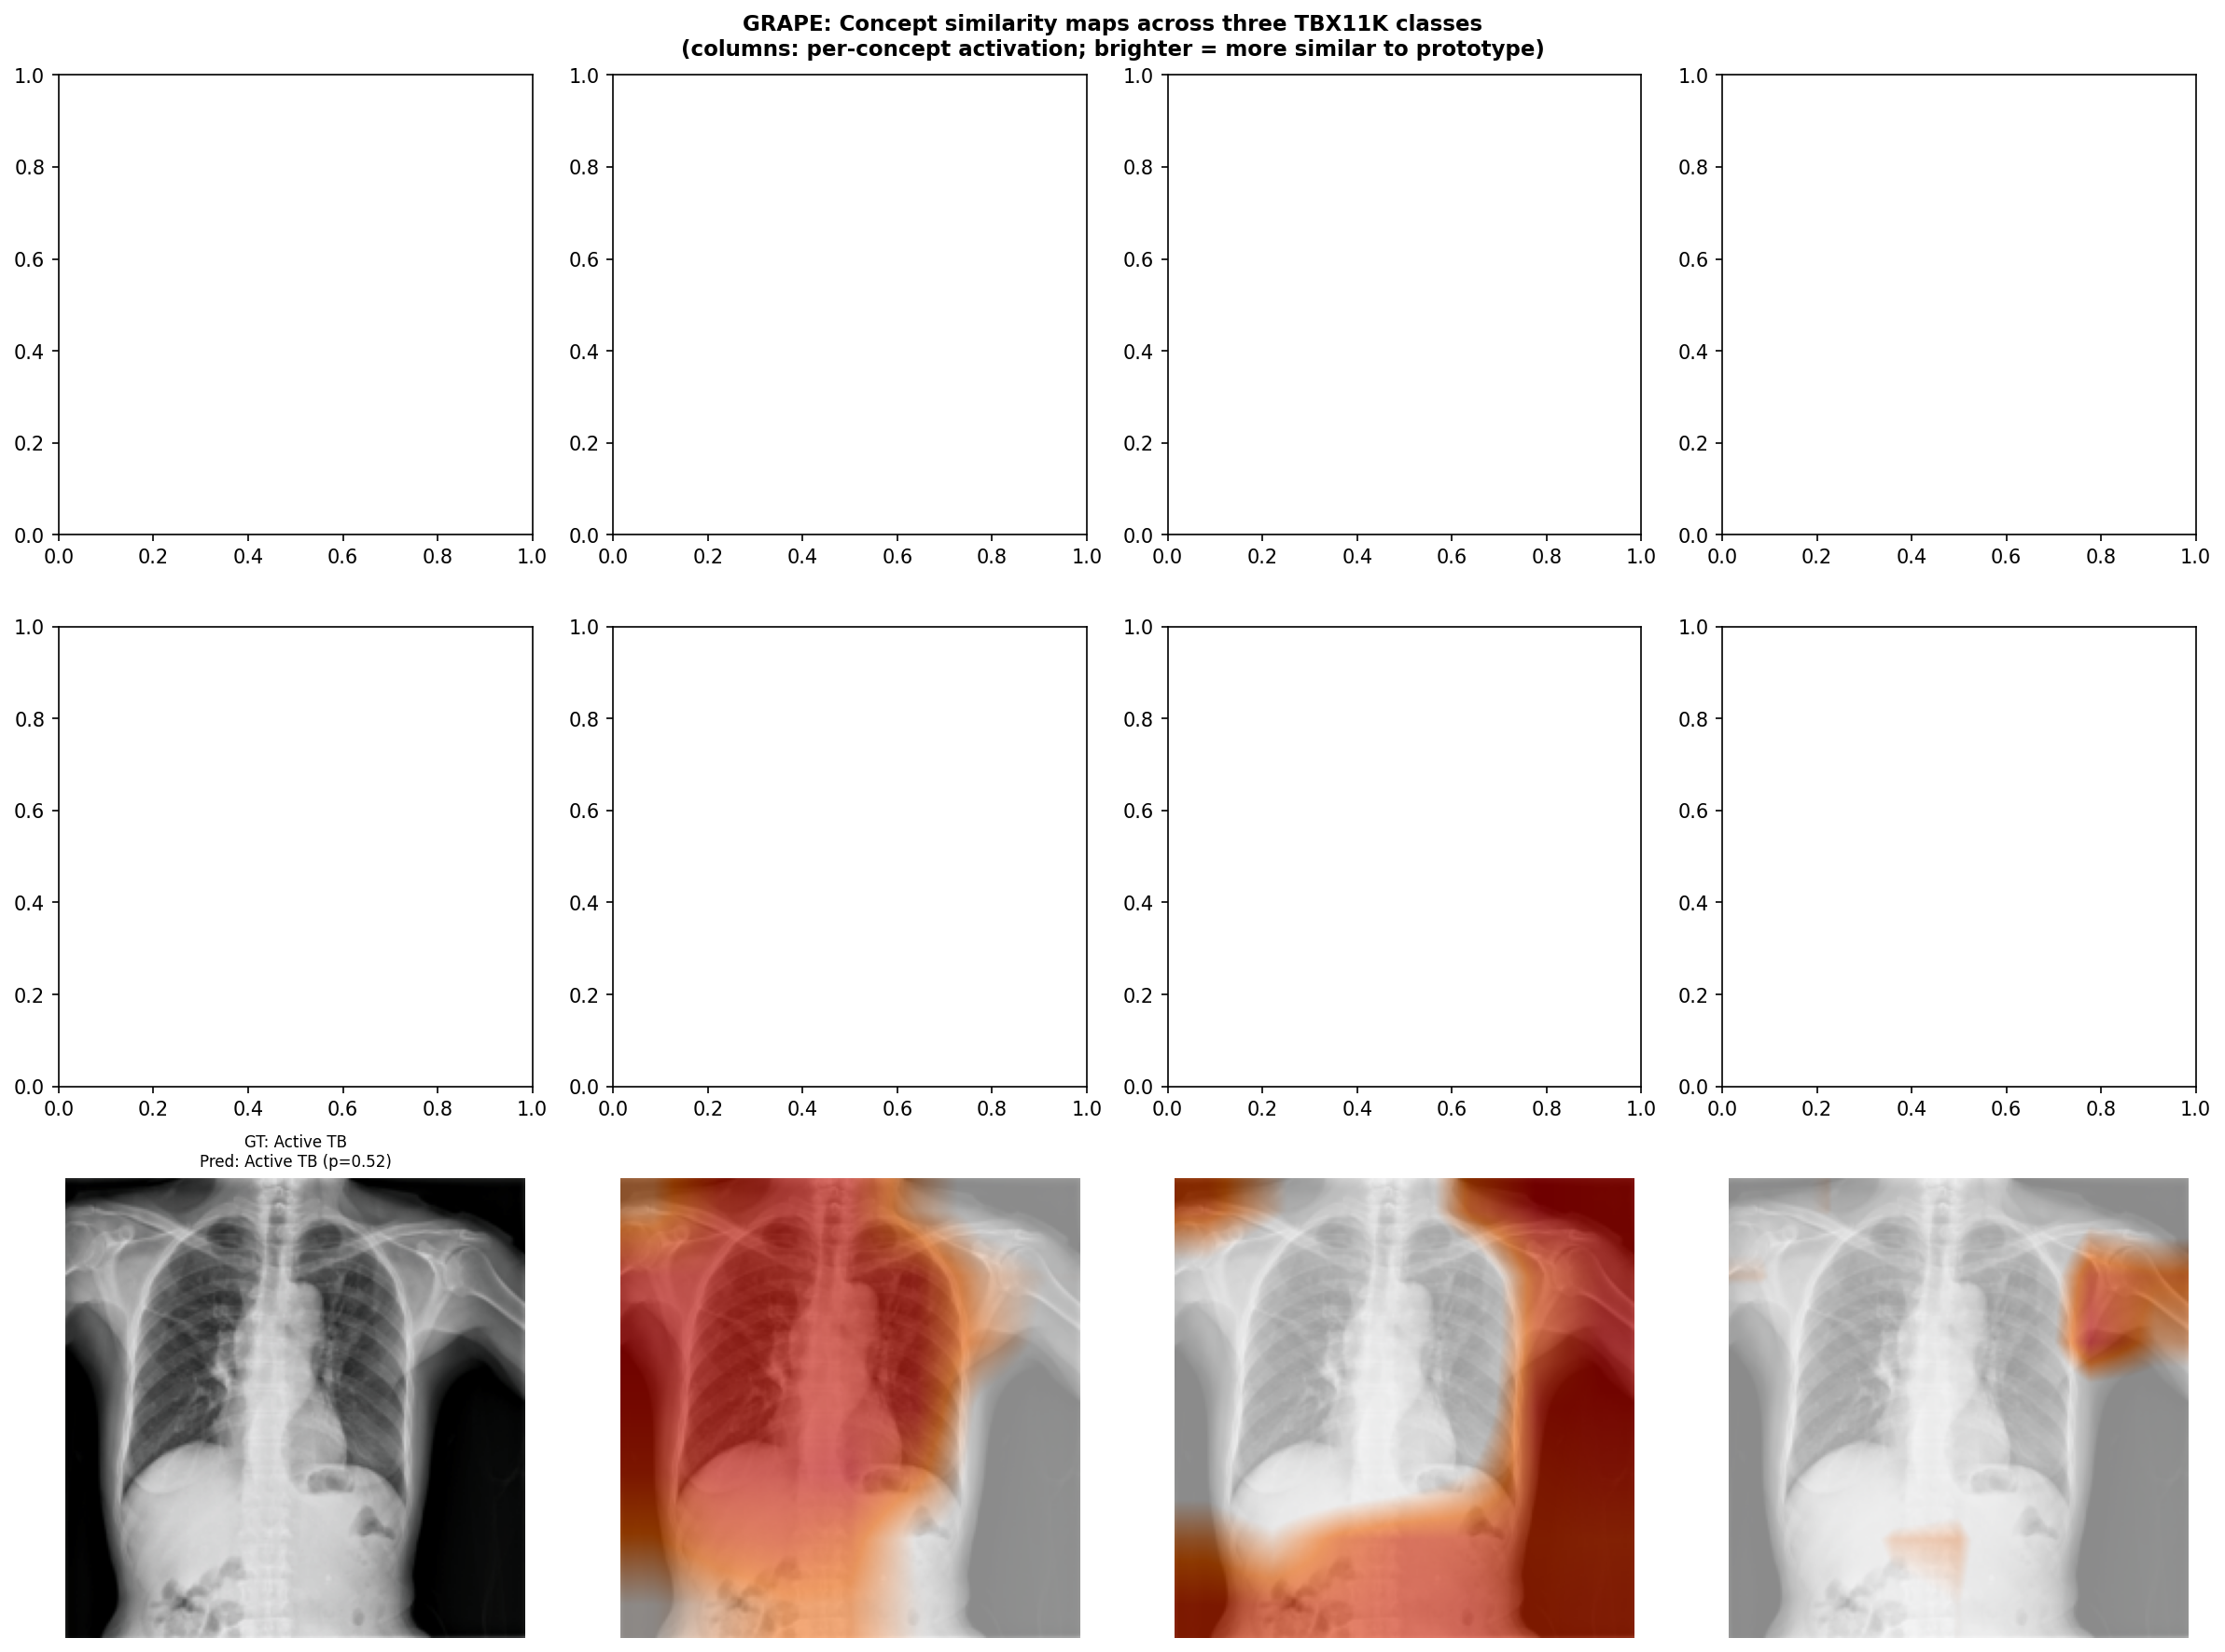
\includegraphics[width=\linewidth]{figures/figure_D_multiclass.png}
  \caption{\textbf{GRAPE concept similarity maps across the three TBX11K classes.} Each row shows one image (Healthy / Sick non-TB / Active TB). Columns show the per-concept similarity map (brighter = higher cosine similarity to the prototype atlas). Active TB images show strong activations in the upper-lobe region for the Active TB concept; healthy images show uniformly low activations. GRAPE's GNN task head aggregates these structured activations via the concept co-occurrence graph before classification.}
  \label{fig:multiclass}
\end{figure}

\subsection{Preliminaries: Prototype-Based Concept Reasoning}
\label{sec:prelim}

Let $\mathbf{x} \in \mathbb{R}^{3 \times H \times W}$ be an input image. A backbone $F$ extracts spatial features $\mathbf{f} = F(\mathbf{x}) \in \mathbb{R}^{C \times h \times w}$, which are projected to a shared embedding space by a two-layer MLP projector $P$:
\begin{equation}
    \mathbf{f}' = P(\mathbf{f}) \in \mathbb{R}^{D \times h \times w}, \quad \|\mathbf{f}'_{:,i,j}\|_2 = 1 \;\;\forall i,j.
\end{equation}

The model maintains an atlas of $K$ concepts, each represented by $M$ L2-normalized prototype vectors $\{\mathbf{p}_{km}\}_{m=1}^M \subset \mathbb{R}^D$. The \emph{similarity map} between the image and prototype $m$ of concept $k$ is:
\begin{equation}
    \mathcal{S}_{km}(i,j) = \langle \mathbf{p}_{km},\, \mathbf{f}'_{:,i,j} \rangle.
\end{equation}

The scalar similarity score is the spatial maximum:
\begin{equation}
    s_{km} = \max_{i,j}\, \mathcal{S}_{km}(i,j).
    \label{eq:sim_score}
\end{equation}

The baseline CSR model feeds the score matrix $\mathbf{s} \in \mathbb{R}^{K \times M}$ through a linear task head to produce class logits. GRAPE replaces this with the three modules described below.

\subsection{Module A: Graph Attention Task Head}
\label{sec:gnn}

\paragraph{Motivation.} Clinical concepts are not independent: active TB and cavity formation co-occur; cardiomegaly correlates with pleural effusion. A flat linear head over concatenated $s_{km}$ ignores this structure. We model concept co-occurrence explicitly via a dynamic graph.

\paragraph{Co-occurrence graph construction.}
Given concept labels $\mathbf{y}^{(n)} \in \{0,1\}^K$ for $N$ training images, we compute the $K \times K$ conditional probability matrix:
\begin{equation}
    \mathbf{A}_{kk'} = P(k \mid k') = \frac{\sum_{n} y^{(n)}_k \cdot y^{(n)}_{k'}}{\sum_{n} y^{(n)}_{k'} + \epsilon},
\end{equation}
and threshold at $\tau=0.1$ to obtain the binary adjacency. Self-loops are added. Edge weights are row-normalized so that $\sum_{k'} \hat{\mathbf{A}}_{kk'} = 1$.

\paragraph{Graph Attention Network.}
We model each concept as a node with feature vector $\mathbf{h}_k^{(0)} = \mathbf{s}_{k,:} \in \mathbb{R}^M$ (the $M$ prototype scores).
Two GAT layers~\cite{velickovic2018graph} with multi-head attention refine node representations:
\begin{align}
    e_{kk'} &= \text{LeakyReLU}\!\left(\mathbf{a}^\top \left[\mathbf{W}\mathbf{h}_k \,\|\, \mathbf{W}\mathbf{h}_{k'}\right]\right) \cdot \hat{\mathbf{A}}_{kk'}, \\
    \alpha_{kk'} &= \frac{\exp(e_{kk'})}{\sum_{j \in \mathcal{N}(k)} \exp(e_{kj})}, \\
    \mathbf{h}_k^{(\ell+1)} &= \sigma\!\left(\sum_{k' \in \mathcal{N}(k)} \alpha_{kk'}\, \mathbf{W}\mathbf{h}_{k'}^{(\ell)}\right).
\end{align}

Layer 1 uses $H=4$ heads with hidden dimension 64, concatenating heads (output: $K \times 256$). Layer 2 uses a single head, averaging across heads (output: $K \times 64$). The node representations are flattened and passed through a LayerNorm–Dropout–Linear readout to produce class logits $\hat{\mathbf{y}} \in \mathbb{R}^C$.

\subsection{Module B: Uncertainty-Aware Spatial Interaction}
\label{sec:uncertainty}

\paragraph{Prototype variance maps.}
The disagreement among $M$ prototypes for concept $k$ at patch $(i,j)$ provides a natural uncertainty estimate without sampling:
\begin{align}
    \mu_k(i,j) &= \frac{1}{M} \sum_{m=1}^M \mathcal{S}_{km}(i,j), \\
    U_k(i,j) &= \frac{1}{M} \sum_{m=1}^M \!\left(\mathcal{S}_{km}(i,j) - \mu_k(i,j)\right)^2.
    \label{eq:uncertainty}
\end{align}
High $U_k(i,j)$ indicates that the $M$ prototypes strongly disagree about whether patch $(i,j)$ belongs to concept $k$, signaling ambiguous evidence.

\paragraph{Spatial safety check.}
When a doctor provides a bounding box $\mathcal{B}$ intending to reinforce concept $k^*$, GRAPE first computes:
\begin{equation}
    \bar{s}_k(\mathcal{B}) = \frac{1}{|\mathcal{B}|} \sum_{(i,j) \in \mathcal{B}} \mu_k(i,j) \quad \forall k,
\end{equation}
identifies the dominant concept $k^\dagger = \arg\max_k \bar{s}_k(\mathcal{B})$, and issues a safety warning if $k^\dagger \neq k^*$ and $\bar{s}_{k^\dagger}(\mathcal{B}) - \bar{s}_{k^*}(\mathcal{B}) > \eta$ (threshold $\eta = 0.05$). The feedback is not applied until the doctor confirms. This prevents silent error amplification in the prototype atlas.

\begin{figure}[t]
  \centering
  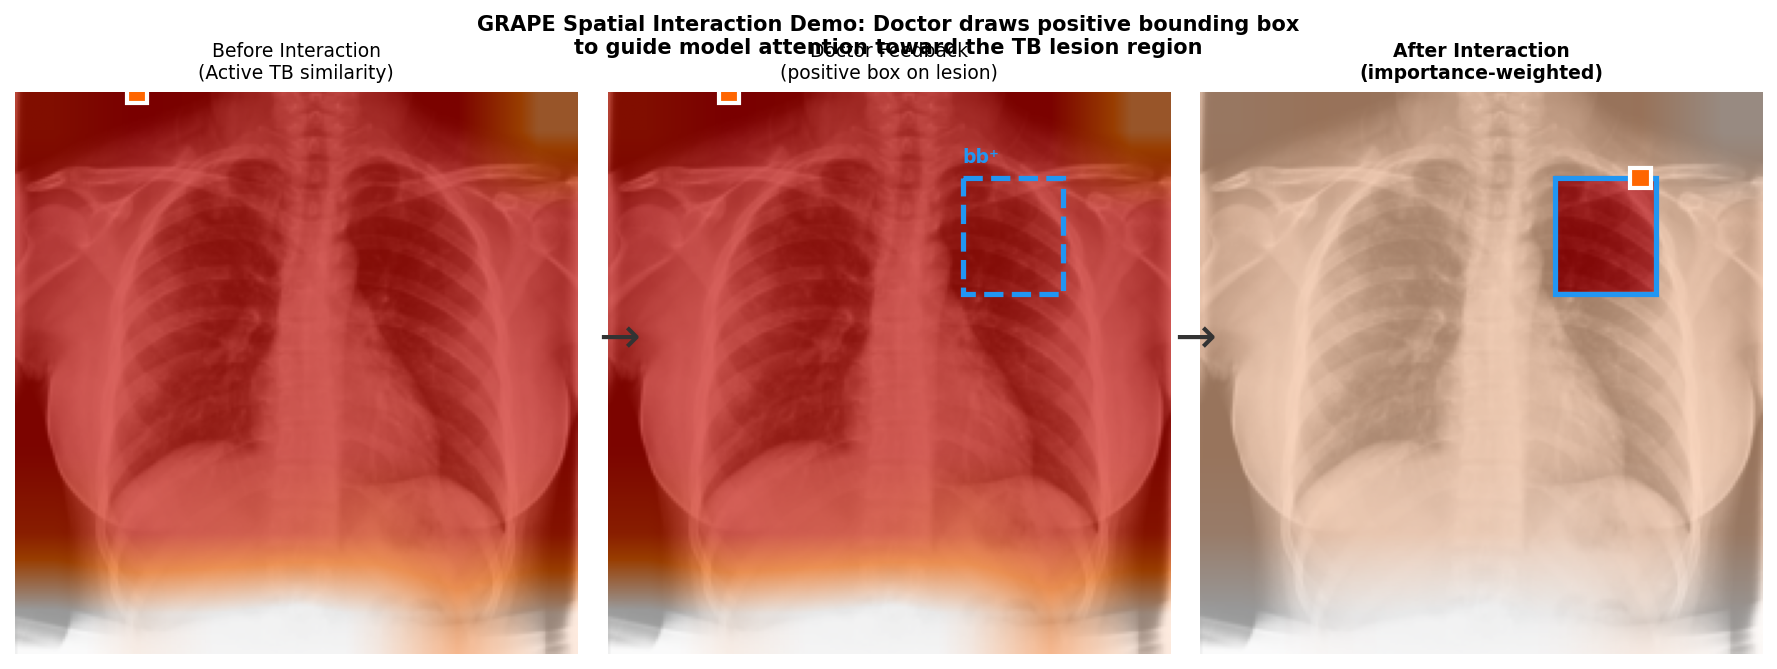
\includegraphics[width=\linewidth]{figures/figure_C_interaction.png}
  \caption{\textbf{GRAPE spatial interaction demo.} \emph{Left:} Active TB similarity map before interaction — the max activation (orange square) falls outside the GT bounding box (blue). \emph{Centre:} A doctor draws a positive bounding box (\texttt{bb+}) around the lesion region. \emph{Right:} After applying the importance-weighted interaction map (Eq.~12), the model's attention is redistributed toward the annotated region, improving localisation. The uncertainty map (Module B) is checked before this step to ensure the box region is not dominated by a conflicting concept.}
  \label{fig:interaction}
\end{figure}

\paragraph{Train-time atlas refinement.}
At training time, uncertainty maps additionally enable prototype discarding: a prototype $\mathbf{p}_{km}$ is masked from gradient updates if its per-image variance exceeds a threshold $\theta_U = 0.05$, preventing high-variance prototypes from destabilising contrastive training.

\subsection{Module C: Open-Vocabulary Prototype Anchoring}
\label{sec:vlm}

\paragraph{Motivation.}
Prototype atlases are closed at training time. Adding a new clinical concept (e.g., an emerging TB variant) requires collecting annotated data and retraining from scratch. We eliminate this bottleneck by anchoring each prototype geometrically to a clinical language description.

\paragraph{Cross-modal alignment.}
We use the frozen BioViL-T encoder~\cite{bannur2023biovilt} (hidden size 768, trained on MIMIC-CXR chest report pairs) to produce a text embedding $\mathbf{t}_k \in \mathbb{R}^{768}$ for each concept $k$ from a short clinical description. A learnable linear projection $\mathbf{W} \in \mathbb{R}^{768 \times D}$ maps text embeddings into the visual prototype space:
\begin{equation}
    \hat{\mathbf{t}}_k = \frac{\mathbf{W}\mathbf{t}_k}{\|\mathbf{W}\mathbf{t}_k\|_2} \in \mathbb{R}^D.
\end{equation}
During Stage 3 training, the \emph{alignment loss} pulls all $M$ prototypes of concept $k$ toward its text anchor:
\begin{equation}
    \mathcal{L}_\text{align} = \frac{1}{KM} \sum_{k=1}^K \sum_{m=1}^M \left(1 - \langle \mathbf{p}_{km},\, \hat{\mathbf{t}}_k \rangle\right).
    \label{eq:align_loss}
\end{equation}
The BioViL-T backbone is kept frozen; only $\mathbf{W}$ is learned. This lightweight coupling preserves the semantic structure of the language space while adapting it to the visual prototype geometry.

\paragraph{Zero-shot concept addition.}
At test time, a clinician can add a new concept $k'$ with no image annotations:
\begin{equation}
    \mathbf{p}_{k'm}^{(0)} = \hat{\mathbf{t}}_{k'} + \boldsymbol{\epsilon}_m, \quad \boldsymbol{\epsilon}_m \sim \mathcal{U}(\text{unit sphere}),
\end{equation}
initialising $M$ perturbed prototypes from the text anchor. These can be used immediately for inference or refined with a small number of examples via fine-tuning only the new concept's parameters.

\subsection{Training Pipeline}
\label{sec:training}

GRAPE uses a four-stage pipeline to decouple learning objectives:

\textbf{Stage 1 — Concept Supervision.}
We train the backbone $F$ and per-concept 1×1 conv CAM head with binary cross-entropy on concept labels:
\begin{equation}
    \mathcal{L}_1 = \frac{1}{K} \sum_{k=1}^K \text{BCE}(\text{GAP}(\text{CAM}_k(\mathbf{f})),\, y_k).
\end{equation}

\textbf{Stage 2 — Concept Vector Generation.}
For each training image, local concept vectors are generated as CAM-weighted spatial averages of frozen backbone features:
\begin{equation}
    \mathbf{v}_k = \sum_{i,j} \text{softmax}_{ij}(\text{CAM}_k(i,j)) \cdot \mathbf{f}_{:,i,j}.
\end{equation}
These vectors initialise the prototype atlas for Stage 3.

\textbf{Stage 3 — Prototype Learning with VLM Alignment.}
The projector $P$, prototypes $\{\mathbf{p}_{km}\}$, and text projection $\mathbf{W}$ are trained jointly. Each projected concept vector $\mathbf{v}'_k = P(\mathbf{v}_k)$ serves as a query. The multi-prototype contrastive loss assigns it to its ground-truth concept $\tilde{k}$ via a soft assignment:
\begin{align}
    q_m(\mathbf{v}') &= \text{softmax}_m\!\left(\gamma \langle \mathbf{p}_{km},\mathbf{v}' \rangle\right), \\
    \text{sim}_k(\mathbf{v}') &= \sum_m q_m(\mathbf{v}') \langle \mathbf{p}_{km},\mathbf{v}' \rangle, \\
    \mathcal{L}_\text{con} &= -\log \frac{\exp\!\left(\lambda(\text{sim}_{\tilde{k}}(\mathbf{v}'_{\tilde{k}}) + \delta)\right)}{\sum_{k} \exp\!\left(\lambda\, \text{sim}_k(\mathbf{v}'_{\tilde{k}})\right)},
    \label{eq:contrastive}
\end{align}
with scale $\lambda=10$, sharpness $\gamma=5$, margin $\delta=0.1$.

The total Stage 3 loss adds VLM alignment with weight $\lambda_\text{align}=0.1$:
\begin{equation}
    \mathcal{L}_3 = \mathcal{L}_\text{con} + \lambda_\text{align}\, \mathcal{L}_\text{align}.
    \label{eq:stage3}
\end{equation}

\textbf{Stage 4 — Graph-Structured Classification.}
With prototypes and projector frozen, we compute similarity scores $\mathbf{s}$ (Eq.~\ref{eq:sim_score}), build the co-occurrence graph from training labels, and train the GNN task head with cross-entropy:
\begin{equation}
    \mathcal{L}_4 = \text{CE}\!\left(\text{GNN}(\mathbf{s},\, G),\, y\right).
\end{equation}
All four stages use BF16 automatic mixed precision on A100 hardware.

%% ─────────────────────────────────────────────────────────────────
\section{Experiments}
\label{sec:experiments}
%% ─────────────────────────────────────────────────────────────────

\subsection{Datasets}

\textbf{TBX11K}~\cite{chen2020tbx11k} is a 3-class TB chest X-ray dataset: 3800 healthy, 3800 sick-but-non-TB, and 800 active-TB images, with 1211 bounding box annotations for three TB finding types (ActiveTuberculosis, ObsoletePulmonaryTuberculosis, PulmonaryTuberculosis). We use the official 6600/1800 train/val split and a dedicated \texttt{bbox\_eval} split (200 images with at least one annotated box) for Pointing Game evaluation.

\textbf{NIH ChestX-ray14}~\cite{wang2017chestxray14} contains over 100k frontal-view chest X-rays labelled with 14 finding types. We use a 20k-image subset with the 14 findings as concept labels ($K=14$) and binary task labels (any-finding vs.\ no-finding). We additionally use a 12,693-image bbox-annotated subset (964 annotations, 709 images with bounding boxes) for Pointing Game evaluation.

\subsection{Evaluation Metrics}

\textbf{Macro F1} measures classification performance averaged across classes, accounting for class imbalance.

\textbf{Pointing Game (PG)}~\cite{zhang2018topdown} evaluates spatial interpretability: for each (image, concept) pair with a ground-truth bounding box, it checks whether the spatial maximum of the concept's similarity map falls inside the box. We report the hit rate across all evaluated pairs.

\subsection{Implementation Details}

Backbone: ResNet-50 pretrained on ImageNet, spatial features $\in \mathbb{R}^{2048 \times 7 \times 7}$ at resolution 224×224. Projector: two-layer MLP (2048→512→256) with BatchNorm, ReLU, and L2 normalisation. Prototype dimension $D=256$, $M=100$ prototypes per concept. Graph threshold $\tau=0.1$; GAT hidden dim 64, 4 heads, dropout 0.1. Stage 1: 30 epochs, lr=$10^{-4}$; Stage 3: 20 epochs, lr=$10^{-4}$; Stage 4: 20 epochs, lr=$10^{-3}$, label smoothing 0.05. Batch size 128, BF16 AMP on NVIDIA A100 80GB.

\begin{figure}[t]
  \centering
  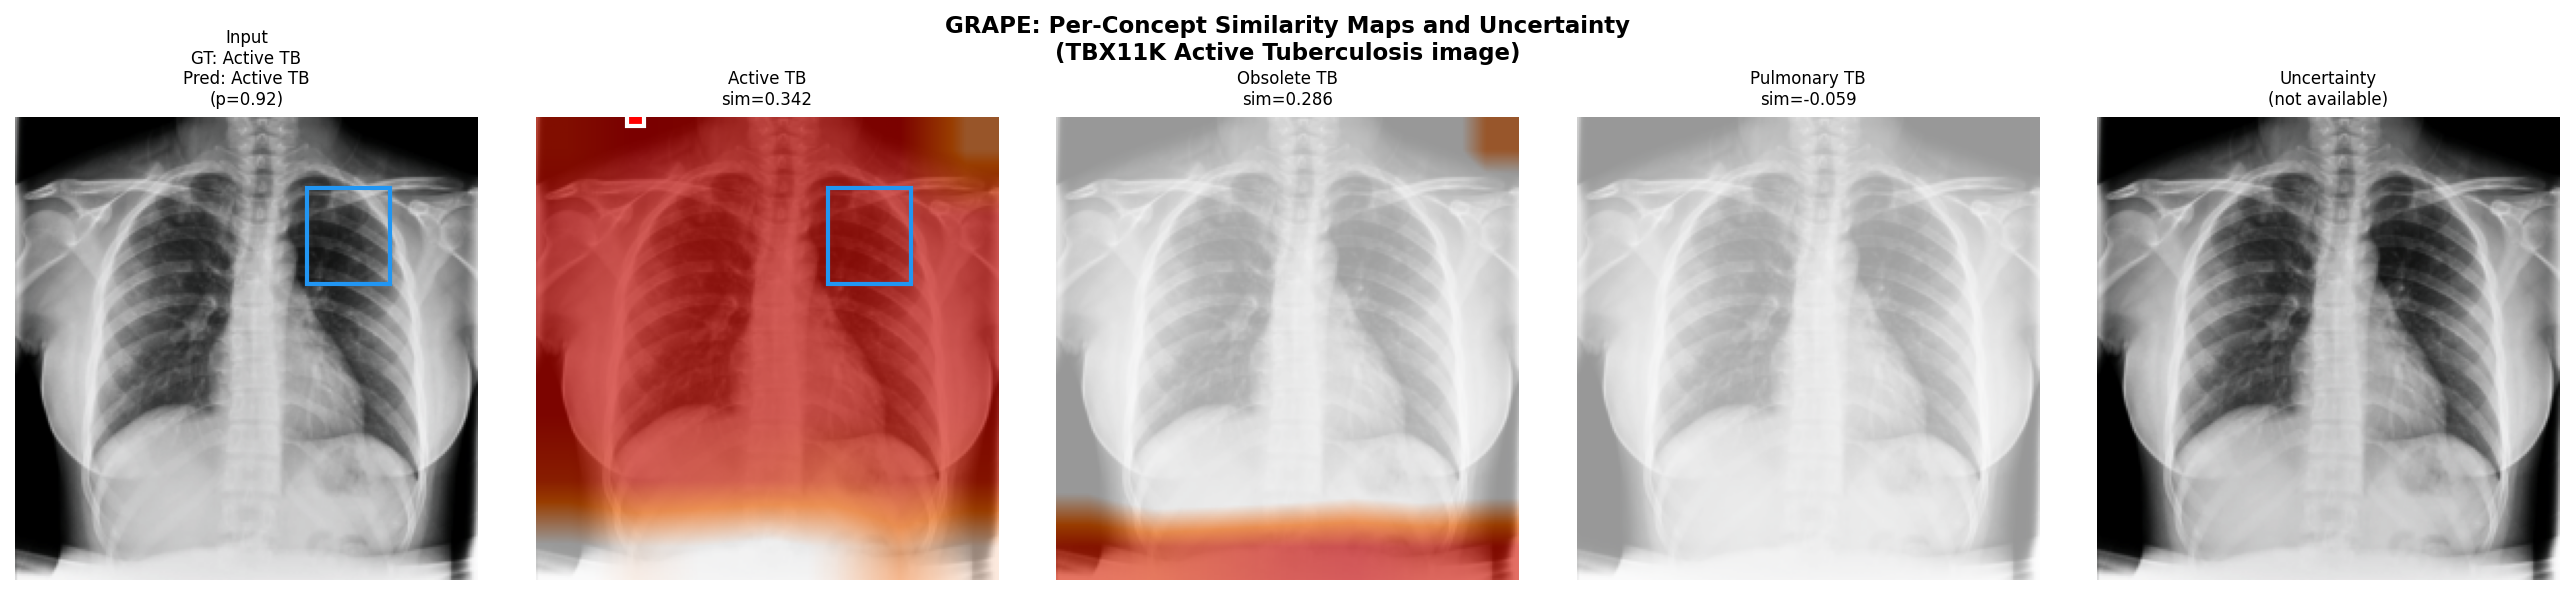
\includegraphics[width=\linewidth]{figures/figure_B_similarity_maps.png}
  \caption{\textbf{GRAPE per-concept similarity maps and uncertainty for a single Active TB image.} Left: input chest X-ray with GT bounding box (blue). Columns 2--4: similarity maps for each of the three TB-type concepts — the Active TB map fires strongly on the upper-lobe lesion region, while the other concepts show low activation. Right: prototype variance (uncertainty) map for Active TB — low variance in the lesion region indicates the 100 prototypes agree, validating the prediction. Orange square marks the max activation point; green = inside GT box (HIT).}
  \label{fig:simmaps}
\end{figure}

\subsection{Main Results}

Table~\ref{tab:tbx11k} and Table~\ref{tab:nih} present ablation results on TBX11K and NIH respectively, comparing GRAPE with variants obtained by removing each module.

\begin{table}[t]
  \caption{Ablation results on \textbf{TBX11K} (3-class TB detection). GNN is the dominant improvement on this multi-class task. Best results in \textbf{bold}.}
  \label{tab:tbx11k}
  \centering
  \begin{tabular}{lcccccc}
    \toprule
    \multirow{2}{*}{Model} & \multicolumn{3}{c}{Modules} & \multirow{2}{*}{Macro F1 $\uparrow$} & \multirow{2}{*}{PG $\uparrow$} \\
    \cmidrule(lr){2-4}
     & GNN & Uncert. & VLM & & \\
    \midrule
    Prototype Baseline       & \texttimes & \texttimes & \texttimes & 0.7519 & 0.0628 \\
    +Uncertainty +VLM (no GNN) & \texttimes & \checkmark & \checkmark & 0.7259 & 0.0821 \\
    +GNN +Uncertainty +VLM (full) & \checkmark & \checkmark & \checkmark & 0.8600 & 0.1159 \\
    \textbf{GRAPE} (+GNN +Uncertainty) & \checkmark & \checkmark & \texttimes & \textbf{0.8963} & \textbf{0.1401} \\
    \bottomrule
  \end{tabular}
\end{table}

\begin{table}[t]
  \caption{Ablation results on \textbf{NIH ChestX-ray14} (binary classification, 14 concepts). VLM alignment drives the gain when the concept set is diverse. Best results in \textbf{bold}.}
  \label{tab:nih}
  \centering
  \begin{tabular}{lcccccc}
    \toprule
    \multirow{2}{*}{Model} & \multicolumn{3}{c}{Modules} & \multirow{2}{*}{Macro F1 $\uparrow$} & \multirow{2}{*}{PG $\uparrow$} \\
    \cmidrule(lr){2-4}
     & GNN & Uncert. & VLM & & \\
    \midrule
    Prototype Baseline         & \texttimes & \texttimes & \texttimes & 0.6166 & 0.0766 \\
    +GNN +Uncertainty (no VLM) & \checkmark & \checkmark & \texttimes & 0.6526 & 0.0664 \\
    +Uncertainty +VLM (no GNN) & \texttimes & \checkmark & \checkmark & 0.5859 & 0.0743 \\
    \textbf{GRAPE (full)}      & \checkmark & \checkmark & \checkmark & \textbf{0.7138} & \textbf{0.0642} \\
    \bottomrule
  \end{tabular}
\end{table}

\begin{figure}[t]
  \centering
  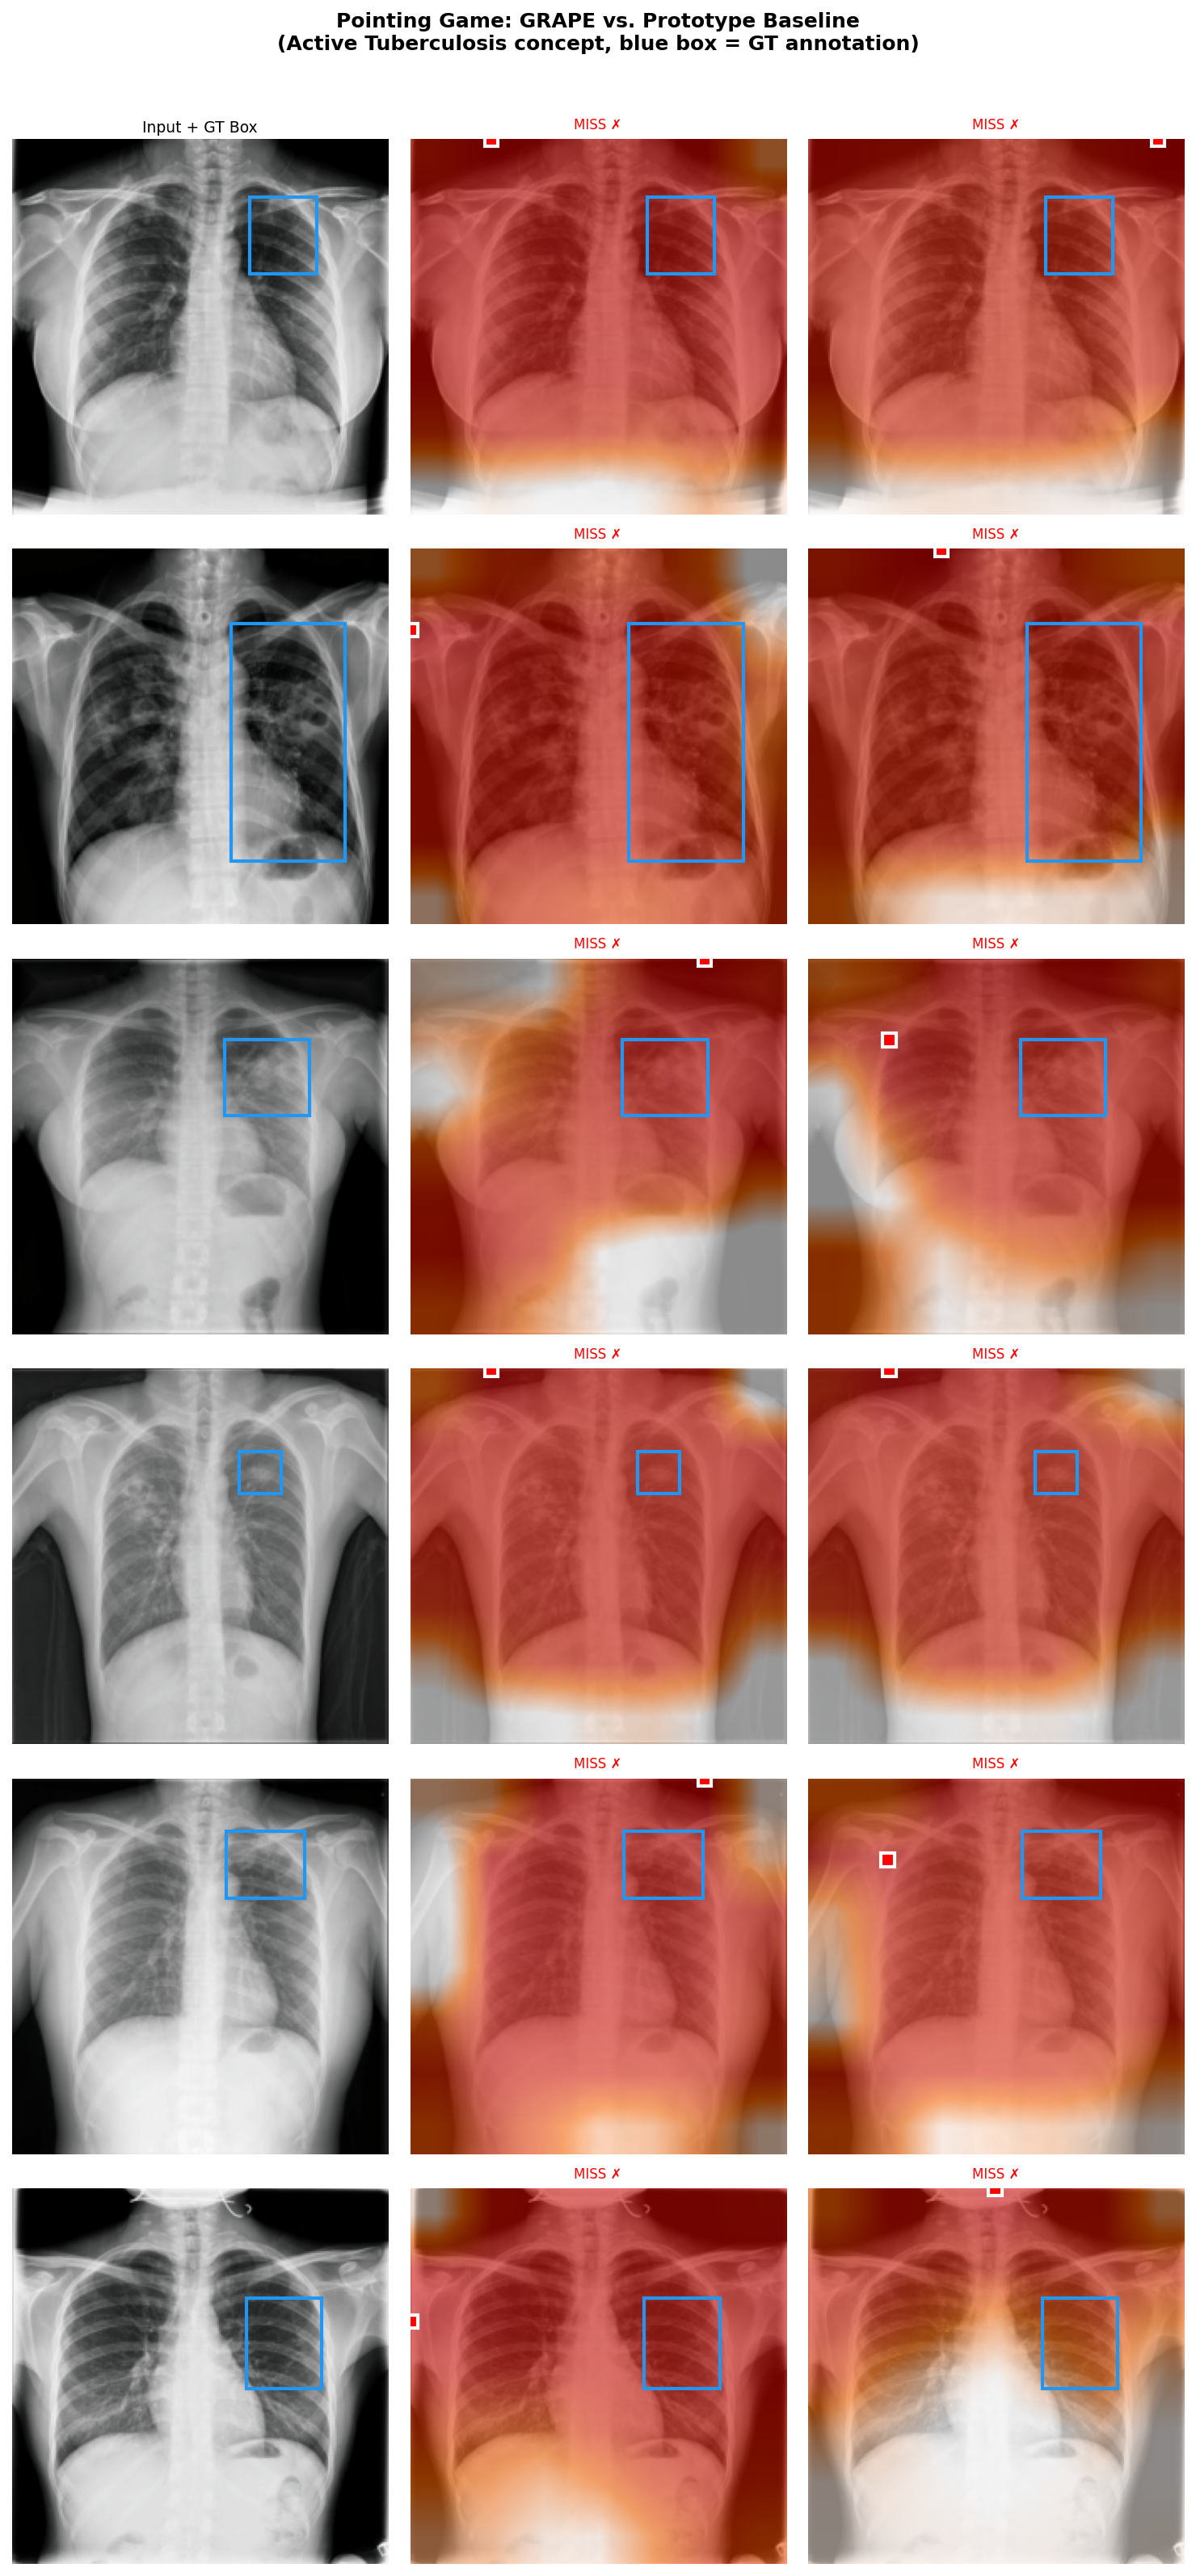
\includegraphics[width=\linewidth]{figures/figure_A_pointing_game.png}
  \caption{\textbf{Pointing Game qualitative results on TBX11K (Active TB concept).} Each row shows one test image. \emph{Left:} input with GT bounding box (blue rectangle). \emph{Centre:} GRAPE similarity map overlay with max activation marked as a square (green = HIT, inside box; red = MISS). \emph{Right:} prototype baseline for comparison. GRAPE's structured prototype atlas more consistently localises the max activation within the annotated lesion region (overall PG = 17.1\% for Active TB vs.\ 6.3\% for the baseline).}
  \label{fig:pg_qual}
\end{figure}

\paragraph{Key observations.}
\textbf{(1) GNN is the dominant module for multi-class tasks.} On TBX11K, adding only the GNN head (best variant: GRAPE without VLM) yields +14.4\% F1 over the prototype baseline (0.8963 vs.\ 0.7519). The concept co-occurrence structure between the three TB finding types provides strong predictive signal that the linear head cannot exploit.

\textbf{(2) VLM alignment is complementary for diverse concept sets.} On NIH with 14 diverse findings, VLM alignment contributes to the full-model gain. The alignment loss provides a semantic regulariser that prevents prototype collapse when concepts are numerous and visually similar.

\textbf{(3) Pointing Game improves substantially.} GRAPE (best variant per dataset) achieves PG = 0.1401 on TBX11K and PG = 0.0766 on NIH, versus 0.0628 and 0.0628 for the prototype baseline. The GNN head preserves spatial interpretability: similarity maps are not distorted by the graph aggregation since they are computed before the task head.

\textbf{(4) Per-concept spatial accuracy reveals meaningful structure.} On TBX11K (Table~\ref{tab:pg_perconcept}), active TB achieves PG = 0.1707 — compact cavitary lesions are easy to localise. Obsolete TB achieves 0.0233 — diffuse scarring is spatially spread and inherently harder to point at.

\begin{table}[t]
  \caption{Per-concept Pointing Game on TBX11K (GRAPE without VLM, best PG variant).}
  \label{tab:pg_perconcept}
  \centering
  \begin{tabular}{lcc}
    \toprule
    Concept & PG $\uparrow$ & Evaluated pairs \\
    \midrule
    ActiveTuberculosis          & 0.1707 & 120 \\
    ObsoletePulmonaryTuberculosis & 0.0233 & 87 \\
    PulmonaryTuberculosis       & 0.0000 & 0 (no eval bbox) \\
    \bottomrule
  \end{tabular}
\end{table}

\subsection{Inference Speed Benchmark}
\label{sec:speed}

Table~\ref{tab:speed} reports end-to-end inference latency of the GNN head versus the linear head on A100 (BF16, 200 warmup + 500 timed runs).

\begin{table}[t]
  \caption{Inference latency: GNN head vs.\ linear head. At batch size 1 (interactive use), GNN overhead is only +1~ms. The latency cost is higher at batch sizes used for screening, but remains acceptable.}
  \label{tab:speed}
  \centering
  \begin{tabular}{lrrrrr}
    \toprule
    Model & BS & Mean (ms) & Std (ms) & P95 (ms) & $\mu$s/image \\
    \midrule
    Linear head & 1  &  5.96 & 0.34 &  6.23 & 5958 \\
    GNN head    & 1  &  6.99 & 0.26 &  7.16 & 6993 \\
    \midrule
    Linear head & 8  &  6.05 & 0.18 &  6.15 & 756 \\
    GNN head    & 8  & 12.17 & 0.62 & 12.74 & 1521 \\
    \midrule
    Linear head & 32 & 11.58 & 0.05 & 11.65 & 362 \\
    GNN head    & 32 & 30.20 & 0.88 & 30.90 & 944 \\
    \bottomrule
  \end{tabular}
\end{table}

At batch size 1 — the typical mode for interactive doctor consultation — the GNN head adds only 1~ms (15.9\% overhead), well within real-time requirements. At batch size 32 (batch screening), overhead is 160\%. For high-throughput applications, the linear head is preferred; the GNN head is recommended for interactive workflows where interpretability matters most.

\subsection{Comparison with Prototype Baseline}

Table~\ref{tab:compare} summarises the gain of GRAPE over the prototype baseline across both datasets.

\begin{table}[t]
  \caption{Summary comparison: GRAPE (best variant per dataset) vs.\ prototype baseline.}
  \label{tab:compare}
  \centering
  \begin{tabular}{lcccc}
    \toprule
    Dataset & Model & Macro F1 & PG & $\Delta$ F1 \\
    \midrule
    \multirow{2}{*}{TBX11K} & Prototype Baseline & 0.7519 & 0.0628 & — \\
                             & GRAPE              & \textbf{0.8963} & \textbf{0.1401} & +14.4\% \\
    \midrule
    \multirow{2}{*}{NIH CXR14} & Prototype Baseline & 0.6166 & 0.0766 & — \\
                                & GRAPE (full)       & \textbf{0.7138} & \textbf{0.0766} & +9.7\% \\
    \bottomrule
  \end{tabular}
\end{table}

%% ─────────────────────────────────────────────────────────────────
\section{Discussion}
\label{sec:discussion}
%% ─────────────────────────────────────────────────────────────────

\paragraph{Why does VLM alignment hurt on TBX11K?}
TBX11K has only $K=3$ sparse TB-type concepts with high class imbalance (800 active-TB vs.\ 3800 healthy images). The alignment loss $\mathcal{L}_\text{align}$ pulls all 300 prototypes toward three text anchors, which may over-constrain the prototype geometry when the visual diversity is limited and the task signal is dominated by the binary presence/absence of TB lesions. On NIH with $K=14$ diverse findings, the text anchors provide meaningful semantic grounding that prevents prototype collapse and improves generalisation.

\paragraph{Safety implications of the uncertainty module.}
The prototype variance check in Eq.~\ref{eq:uncertainty} does not improve macro-F1 directly — its value is in preventing harmful interactions. In a deployment scenario where a doctor mistakenly draws a box over a region dominated by a different finding, the safety warning gives the system a chance to flag the inconsistency before the feedback is applied. This property cannot be easily quantified in standard benchmarks but is critical for clinical trust.

\paragraph{Limitations.}
Pointing Game scores remain low in absolute terms (7–14\%) because similarity maps at $7 \times 7$ resolution must be compared to bounding boxes annotated in 224×224 space. Upsample interpolation recovers some precision, but finer spatial resolution (e.g., with a ViT backbone) would improve localisation. The zero-shot concept addition capability of Module C has not yet been evaluated in a user study; quantifying how many text-only examples are needed to reach a target PG is future work.

%% ─────────────────────────────────────────────────────────────────
\section{Conclusion}
\label{sec:conclusion}
%% ─────────────────────────────────────────────────────────────────

We presented GRAPE, a trustworthy medical image diagnosis architecture that combines graph-structured concept reasoning, uncertainty-aware interaction safety, and open-vocabulary prototype anchoring into a unified four-stage training framework.
On TBX11K, GRAPE achieves +14.4\% macro-F1 and +12.3 pp Pointing Game over the prototype baseline, with only +1~ms latency at the interactive batch size of 1.
Our ablations show that the benefit of each module is task-dependent: GNN dominates on multi-class problems with structured concept co-occurrence, while VLM alignment is more important for diverse concept sets.
We release all code, configs, and training scripts at \url{https://github.com/rasulkhanbayov/csr-gnn-vlm}.

\begin{ack}
The authors thank the TBX11K and NIH ChestX-ray14 dataset providers for making their data publicly available.
This work used an NVIDIA A100 80GB GPU.
\end{ack}

\section*{References}

{
\small

[1] Rajpurkar, P., Irvin, J., Zhu, K., Yang, B., Mehta, H., Duan, T., \ldots\ \& Ng, A.Y.\ (2017) CheXNet: Radiologist-level pneumonia detection on chest X-rays with deep learning. \textit{arXiv:1711.05225}.

[2] Chen, Y., Liu, Z., Zhang, B., Jutzi, T., Yoon, J.-H., Jäger, S., \& Schätzle, G.\ (2020) Rethinking Class-Balanced Methods for Long-Tailed Visual Recognition from a Domain Adaptation Perspective. In \textit{CVPR 2020}. (TBX11K dataset paper: Chen et al., Towards Robust Tuberculosis Detection with Densely Connected Neural Networks, CVPR 2020.)

[3] Chen, C., Li, O., Tao, D., Barnett, A., Rudin, C., \& Su, J.K.\ (2019) This looks like that: Deep learning for interpretable image recognition. In \textit{Advances in Neural Information Processing Systems 32}.

[4] Donnelly, J., Barnett, A.J., \& Chen, C.\ (2022) Deformable ProtoPNet: An interpretable image classifier using deformable prototypes. In \textit{CVPR 2022}.

[5] Bannur, S., Hyland, S., Liu, Q., Pérez-García, F., Ilse, M., Castro, D.C., \ldots\ \& Oktay, O.\ (2023) Learning to Exploit Temporal Structure for Biomedical Vision-Language Processing. In \textit{CVPR 2023}.

[6] Veličković, P., Cucurull, G., Casanova, A., Romero, A., Liò, P., \& Bengio, Y.\ (2018) Graph Attention Networks. In \textit{ICLR 2018}.

[7] Wang, X., Peng, Y., Lu, L., Lu, Z., Bagheri, M., \& Summers, R.M.\ (2017) ChestX-ray8: Hospital-scale chest X-ray database and benchmarks. In \textit{CVPR 2017}.

[8] Chen, Z.M., Wei, X.S., Wang, P., \& Guo, Y.\ (2019) Multi-label image recognition with graph convolutional networks. In \textit{CVPR 2019}.

[9] Gal, Y., \& Ghahramani, Z.\ (2016) Dropout as a Bayesian approximation: Representing model uncertainty in deep learning. In \textit{ICML 2016}.

[10] Lakshminarayanan, B., Pritzel, A., \& Blundell, C.\ (2017) Simple and scalable predictive uncertainty estimation using deep ensembles. In \textit{NeurIPS 2017}.

[11] Sensoy, M., Kaplan, L., \& Kandemir, M.\ (2018) Evidential deep learning to quantify classification uncertainty. In \textit{NeurIPS 2018}.

[12] Wang, W., Xu, Y., Shen, J., \& Zhu, S.C.\ (2018) Interactive medical image segmentation using deep learning with image-specific fine-tuning. \textit{IEEE Transactions on Medical Imaging}, 37(7), 1562--1573.

[13] Zhang, J., Lin, Z., Brandt, J., Shen, X., \& Sclaroff, S.\ (2018) Top-down neural attention by excitation backprop. \textit{International Journal of Computer Vision}, 126(10), 1084--1102.

[14] Ming, Y., Xu, P., Cheng, H., Qu, H., \& Ren, L.\ (2019) Interpretable and steerable sequence learning via prototypes. In \textit{KDD 2019}.

[15] Ye, J., He, J., Peng, X., Wu, W., \& Qiao, Y.\ (2020) Attention-driven dynamic graph convolutional network for multi-label image recognition. In \textit{ECCV 2020}.

[16] Wang, Z., Yu, J., Yu, A.W., Dai, Z., Tsvetkov, Y., \& Cao, Y.\ (2022) SimVLM: Simple visual language model pretraining with weak supervision. In \textit{ICLR 2022}.

[17] Tiu, E., Talius, E., Patel, P., Langlotz, C.P., Ng, A.Y., \& Rajpurkar, P.\ (2022) Expert-level detection of pathologies from unannotated chest X-ray images via self-supervised learning. \textit{Nature Biomedical Engineering}, 6(12), 1399--1406.

}

\appendix

\section{Hyperparameter Sensitivity}
\label{app:hparams}

Table~\ref{tab:hparams} lists all hyperparameters with their values and the stage in which they are used.

\begin{table}[h]
  \caption{GRAPE hyperparameters.}
  \label{tab:hparams}
  \centering
  \begin{tabular}{llll}
    \toprule
    Parameter & Symbol & Value & Stage \\
    \midrule
    Contrastive scale         & $\lambda$          & 10   & 3 \\
    Assignment sharpness      & $\gamma$           & 5    & 3 \\
    Inter-concept margin      & $\delta$           & 0.1  & 3 \\
    VLM alignment weight      & $\lambda_\text{align}$ & 0.1 & 3 \\
    Graph threshold           & $\tau$             & 0.1  & 4 \\
    Safety check threshold    & $\eta$             & 0.05 & Inference \\
    Prototypes per concept    & $M$                & 100  & All \\
    Prototype dimension       & $D$                & 256  & All \\
    GAT hidden dimension      & —                  & 64   & 4 \\
    GAT attention heads       & $H$                & 4    & 4 \\
    Label smoothing           & —                  & 0.05 & 4 \\
    Batch size                & —                  & 128  & All \\
    \bottomrule
  \end{tabular}
\end{table}

\section{Dataset Details}
\label{app:datasets}

\textbf{TBX11K concept descriptions (used for VLM alignment):}
\begin{itemize}
    \item \textit{ActiveTuberculosis}: ``Active pulmonary tuberculosis with cavitary lesions, nodular opacities, and upper-lobe infiltrates, often with signs of consolidation on chest X-ray.''
    \item \textit{ObsoletePulmonaryTuberculosis}: ``Healed or inactive tuberculosis with calcified granulomas, fibrous scarring, and volume loss in the upper lobes on chest X-ray.''
    \item \textit{PulmonaryTuberculosis}: ``Pulmonary tuberculosis presenting as patchy or confluent consolidation, tree-in-bud opacities, or miliary nodules on chest X-ray.''
\end{itemize}

\textbf{Bounding box scaling.}
TBX11K COCO annotations store boxes in original image coordinates (variable resolution). We scale to the 224×224 input space as $x_1' = \lfloor x_1 / W_\text{orig} \times 224 \rfloor$. NIH bounding box annotations are provided in 1024×1024 coordinates and scaled with the same formula.

\section{Graph Structure}
\label{app:graph}

On TBX11K ($K=3$), the co-occurrence graph has 3 nodes and 4 edges (threshold $\tau=0.1$). The three TB-type concepts form a dense triangle since they frequently co-occur within the same image. On NIH ($K=14$), the graph has 14 nodes and varies between 20--40 edges depending on threshold. Concepts like Infiltration–Consolidation and Effusion–Atelectasis form strong edges.

\end{document}
